\chapter{Implementation}\label{chap:implementation}

This chapter presents the practical implementation of the system, covering both the client- and server-side components. It begins with an overview of the technologies used, including TypeScript, React, OpenLayers, Go, and Docker. The structure and functionality of the website are then described, with a focus on user interface design, map integration, and communication with the backend. Finally, the server-side implementation is detailed, including the logic behind the forestry road classification algorithm, data processing, and performance optimizations. The chapter provides a technical foundation for understanding how the prototype was built and how its components work together.


\section{Technologies}

This section outlines the key technologies used in the project, explaining both their technical roles and the reasoning behind their selection. Choices were guided by factors such as development efficiency, scalability, and compatibility with the project's geospatial and web-based requirements.

\subsection{TypeScript}

TypeScript\footnote{\url{https://www.typescriptlang.org/}} is a statically typed superset of JavaScript that adds type annotations and other features to improve code quality and maintainability. While JavaScript is popular for both frontend and backend development, it lacks built-in mechanisms to express relationships between components as applications grow. This often leads to runtime errors, many of which are related to incorrect or unexpected types. TypeScript addresses these issues by providing a static type system that checks for such errors during development, before the code is executed. By catching mistakes early and offering better tooling and autocomplete support, TypeScript makes large-scale JavaScript applications easier to develop, refactor, and maintain \cite{typescript_handbook}. 

Although the team had limited prior experience with frontend web development, we aimed to use a language that was both easy to learn and valuable beyond the project, particularly given its widespread use in industry. TypeScript was therefore chosen for the website implementation. It offered full compatibility with JavaScript-based libraries such as OpenLayers and React, while also providing static typing and enhanced code reliability.

\subsection{React}\label{subsec:implementation:technologies:react}

React\footnote{\url{https://react.dev/}} is a JavaScript library designed for rendering user interfaces (UI), where elements on the screen, from buttons to images, can be broken down into small, reusable components. These components are the building blocks of React, allowing you to create, customize, and conditionally display content across your application \cite{react_component}. As an application scales, it becomes increasingly important to manage the state effectively and ensure that data flows smoothly between components. Poorly organized or redundant state can lead to bugs, so React encourages a structured approach to state management. React makes it easy to share states between components \cite{react_managing_state}. 

Using React to develop the website improved both development speed and maintainability that was especially important given the limited timeframe of the project. React's component-based architecture allowed for modular code, easier reuse of UI elements, and better separation of concerns, which contributed to a more efficient workflow.

\subsection{OpenLayers}

OpenLayers\footnote{\url{https://openlayers.org/}} is a JavaScript library used for displaying and interacting with geographic data on web maps. It provides an extensive and well documented set of tools for working with vector and raster data, supporting various formats such as \Gls{geojson}, \Gls{wms}, and \Gls{wfs}. OpenLayers allows developers to create highly customizable and interactive maps with features like layer control, coordinate projections, and dynamic styling \cite{openlayers}.

The website uses OpenLayers to render image layers for \gls{superficial deposit}s, soil moisture, and \gls{frost} depth, and display vector features like forestry roads.  

\subsection{Web Map Service and Web Feature Service}

% NEVNE SPESIFIKKE FUNKSJONER (GetFeatureInfo / GetMap) ?
Web Map Service (\Gls{wms}) and Web Feature Service (\Gls{wfs}) are both standards developed by the Open Geospatial Consortium to facilitate the distribution of geographic information over the web. A WMS generates dynamic maps from spatially referenced data, rendering them as digital images in formats such as PNG, GIF, and JPEG. WMS allows users to request maps that specify geographic regions, desired coordinate systems, and map dimensions. There are also queryable WMS services that enable users to retrieve metadata about the map and its features at specific coordinates. Additionally, \Gls{wms} supports the creation of composite maps by layering different map images, with transparency in formats like PNG and GIF, allowing the underlying maps to be visible \cite{ogc2006wms}.

In contrast, a \Gls{wfs} enables the retrieval of raw geographic data, such as vector features, from a web server. Unlike \Gls{wms}, which provides static map images, \Gls{wfs} allows users to request feature-level data in formats like \Gls{geojson}, enabling more interactive and detailed analyses. \Gls{wfs} supports spatial queries and provides access to vector-based geographic features, such as points, lines, and polygons, which can be used for advanced geospatial analysis and integration into other systems. While \Gls{wms} is ideal for visualizing spatial data, \Gls{wfs} is better suited for manipulating raw geospatial data \cite{ogc2005wfs}.

In the implementation of this product, both \Gls{wms} and \Gls{wfs} are used to visualize and interact with geospatial data. For example, the superficial deposits and frost depth layers utilize \Gls{wms} to display these datasets as map images on the web interface. On the other hand, the forestry road layer is implemented using \Gls{wfs}, providing access to vector-based geographic features as lines. This allows further processing, such as determining \gls{trafficability} or road conditions. Additionally, when querying a single coordinate, the Superficial Deposits layer uses the query operation to retrieve information about the specific location, ensuring that users can obtain feature data at precise geographic points.

\subsection{Go}\label{subsec:implementation:technologies:go}

Go\footnote{\url{https://go.dev/}} is a high-level general purpose programming language that is statically typed and compiled, and offers built-in memory safety, garbage collection, structural typing and concurrency. Go aims to improve programming productivity by combining the efficiency of C\footnote{\url{https://www.c-language.org/}} with the readability and usability of Python\footnote{\url{https://www.python.org/}}. Goroutines, the foundation of concurrency in Go, are lightweight execution threads that run asynchronously and are distributed across multiple CPUs, enabling parallelism in well-structured programs \cite{goproglanguage}.

The implementation of the server in written in Go. Go was chosen due the great concurrency support and group members' personal experiences with the language. Go is particularly well-suited for processing large datasets, such as forest roads, because each road can be processed independently, making it a natural fit for Go's concurrency model. The implementation of the server will be detailed in \autoref{sec:implementation:server}.

\subsection{Docker}\label{subsec:implementation:technologies:docker}

Docker\footnote{\url{https://www.docker.com/}} is a set of technologies that use OS-level virtualization to deliver software in packages called containers. Containerization allows for software applications to run in isolated user spaces, which enables efficient resource utilization, enhanced security, and simplified deployment across different environments \cite{containerizationwikipedia,dockerwikipedia}. Docker containers are built using a Docker image, which is a template that can be stored in a remote registry. Docker images are built using 
Docker Compose, a tool in the Docker suite, is used for defining and running multi-container applications \cite{dockercomposedocs}. The application is deployed with Docker and Docker Compose, this will be detailed in \autoref{chap:deployment}.

\section{Website}

This section describes the implementation of the website, which serves as the main user interface for interacting with map data. It outlines the design and iteration of the user interface, the integration of interactive components using React and OpenLayers, and the implementation of core features such as date selection, dynamic map layers, and trafficability classification.


\begin{comment}
    - Typescript & React (vite/template, code structure?)
        - Template: npm create vite@latest myapp -- --template react-ts
    - OpenLayers
    - GUI-elements
    - Map layers and legends
    - Forestry road vector layer
    - Datepicker / temporal aspect of map layers
\end{comment}

\subsection{User Interface Iterations} % Vet ikke om dette burde være et annet sted?

The \acrfull{ui} underwent several iterations during development before reaching its final form. This section outlines those iterations, beginning with the initial wireframe.

\subsubsection*{Wireframe}

A wireframe was created early in the development process to establish a shared understanding among group members of the website's layout and core functionality. It was developed using Balsamiq, a tool well-suited for quickly creating low-fidelity wireframes. To draw inspiration for the design, several existing map-based websites were reviewed, including SeNorge\footnote{\url{https://www.senorge.no/}} and NIBIO's Kilden\footnote{\url{https://kilden.nibio.no}}.

\autoref{fig:wireframe:closed} shows the basic structure, including the main map view and the date picker component at the top to change the current date. \autoref{fig:wireframe:opened} illustrates the sidebars used to toggle map layers and view their corresponding legends. It also demonstrates how a layer can be activated and queried for additional information, highlighting key interactions envisioned for the final implementation.

The \acrshort{ui} evolved later in the project, for instance, it was decided that only forestry roads would support querying to focus user interaction on the most relevant data and reduce complexity.

\begin{figure}[h]
     \centering
     \begin{subfigure}[b]{0.45\textwidth}
         \centering
         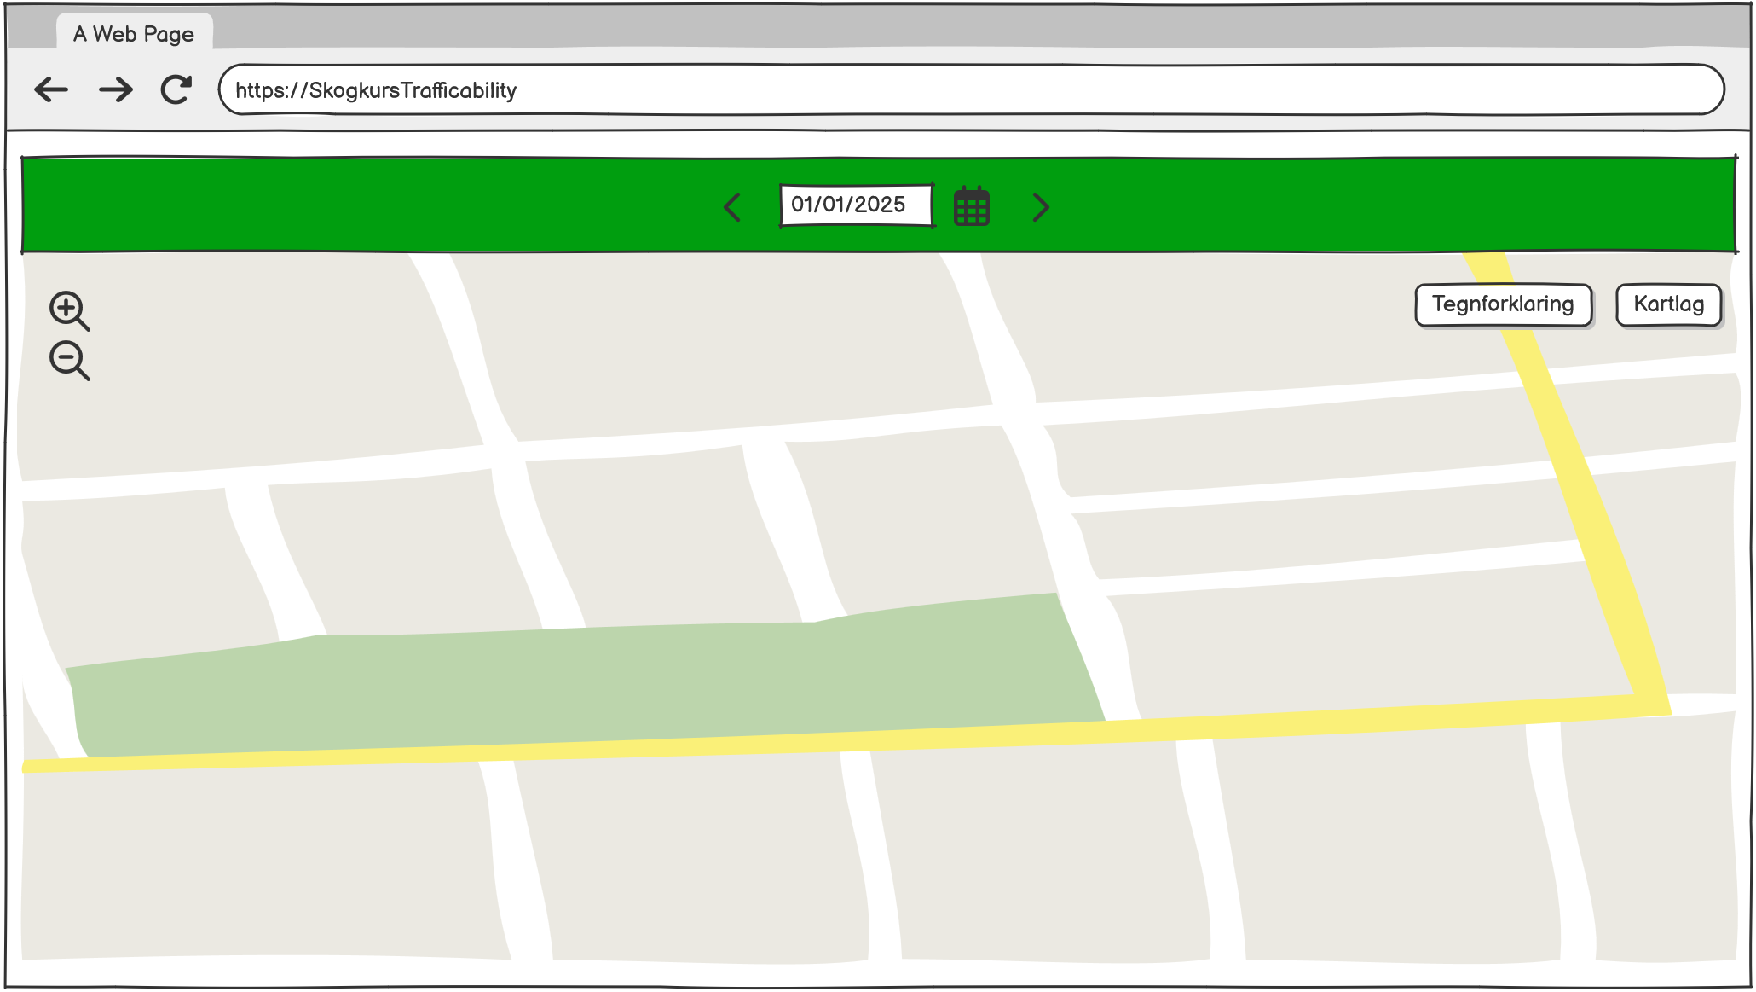
\includegraphics[width=\textwidth]{figures/wireframe_website_sidebars_closed.pdf}
         \caption{Sidebar closed}
         \label{fig:wireframe:closed}
     \end{subfigure}
     \hfill
     \begin{subfigure}[b]{0.45\textwidth}
         \centering
         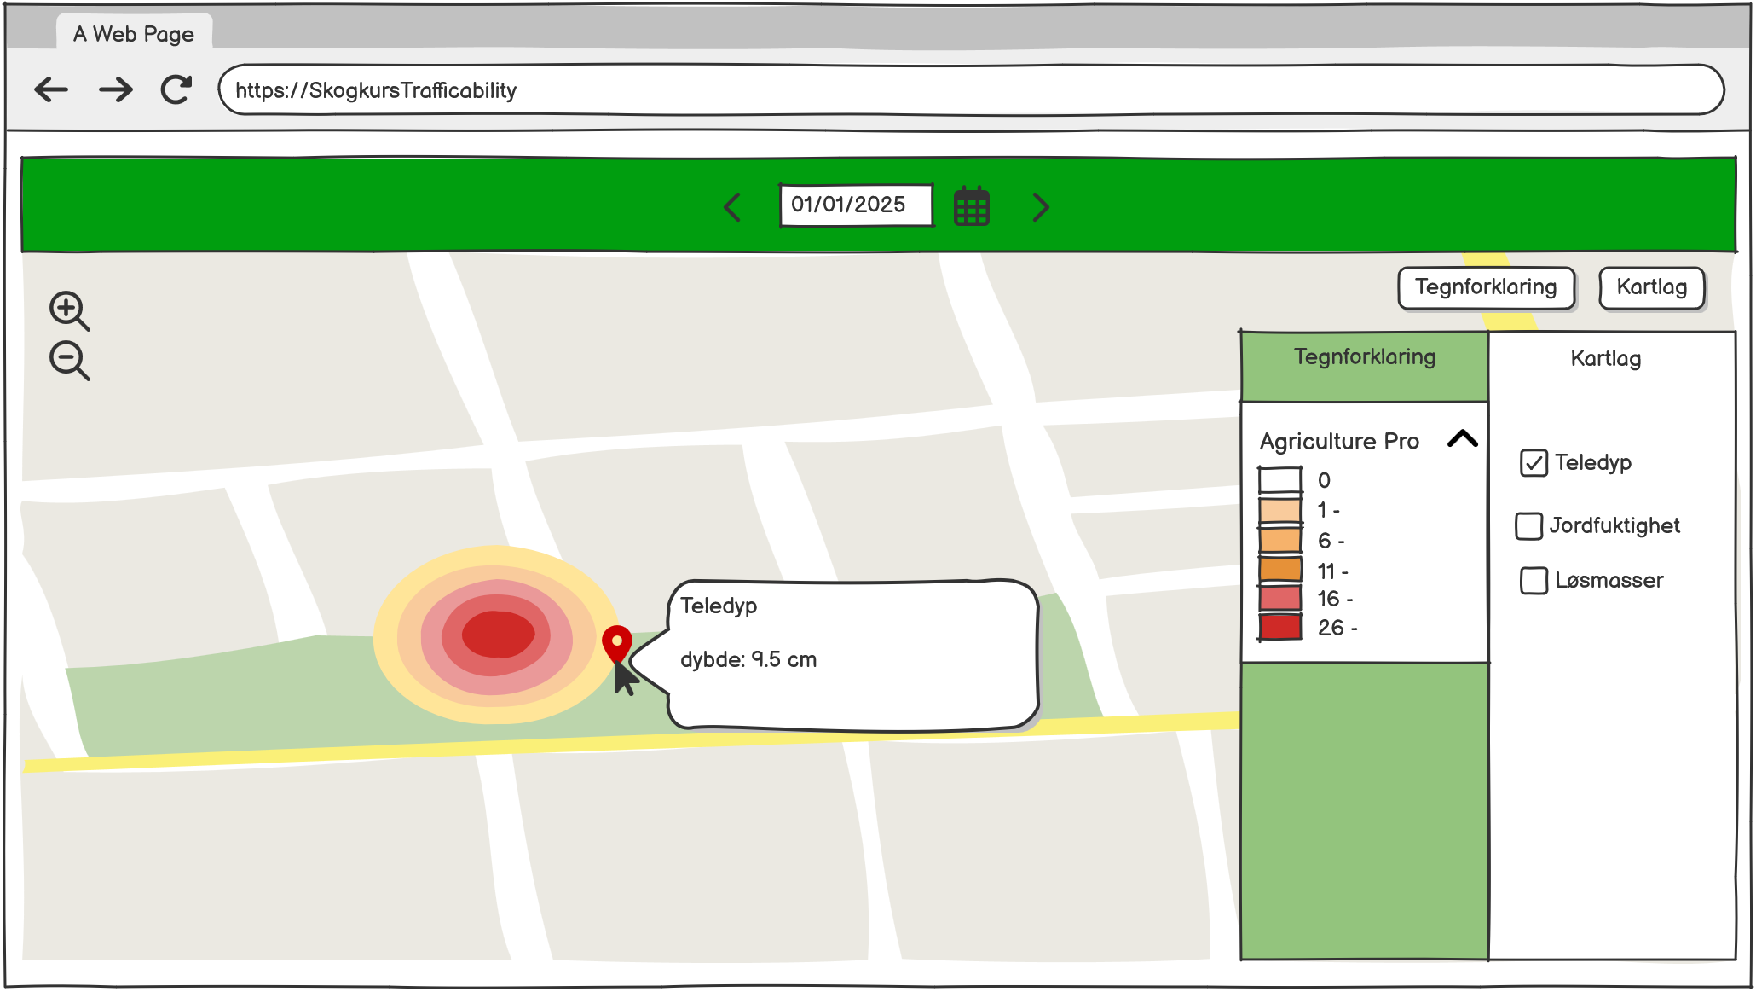
\includegraphics[width=\textwidth]{figures/wireframe_website_sidebars_opened.pdf}
         \caption{Sidebars opened}
         \label{fig:wireframe:opened}
     \end{subfigure}
    \caption{Wireframe of the website}
    \label{fig:wireframe}
\end{figure}

\subsubsection*{Early Iteration}

When we first began implementing the website using OpenLayers, we included several built-in components that seemed potentially useful. One of these was the overview map in the bottom-left corner, which provides a miniature version of the map view. This was helpful for orientation, especially when one or more map layers obscured the base map. We also added a scale line, a common feature in most map applications, to give users a sense of distance and scale.

In the version shown in \autoref{fig:website_layout_v1}, users could query all available map layers, such as the superficial deposit layer. While this functionality was helpful for debugging and comparing data across layers, it introduced unnecessary complexity into the \acrshort{ui}, especially from a user perspective. \textcolor{orange}{Repetering fra forrige section?}

A geolocation button was also included, allowing users to center the map on their current location if they consented to share it. However, when deploying the website on the backend server, we discovered that this feature only works over HTTPS due to browser security policies. Since the feature was not essential to the core functionality, and the project did not include setting up a valid HTTPS certificate, it was ultimately left non-functional in the deployed version.

\begin{figure}[h]
    \centering
    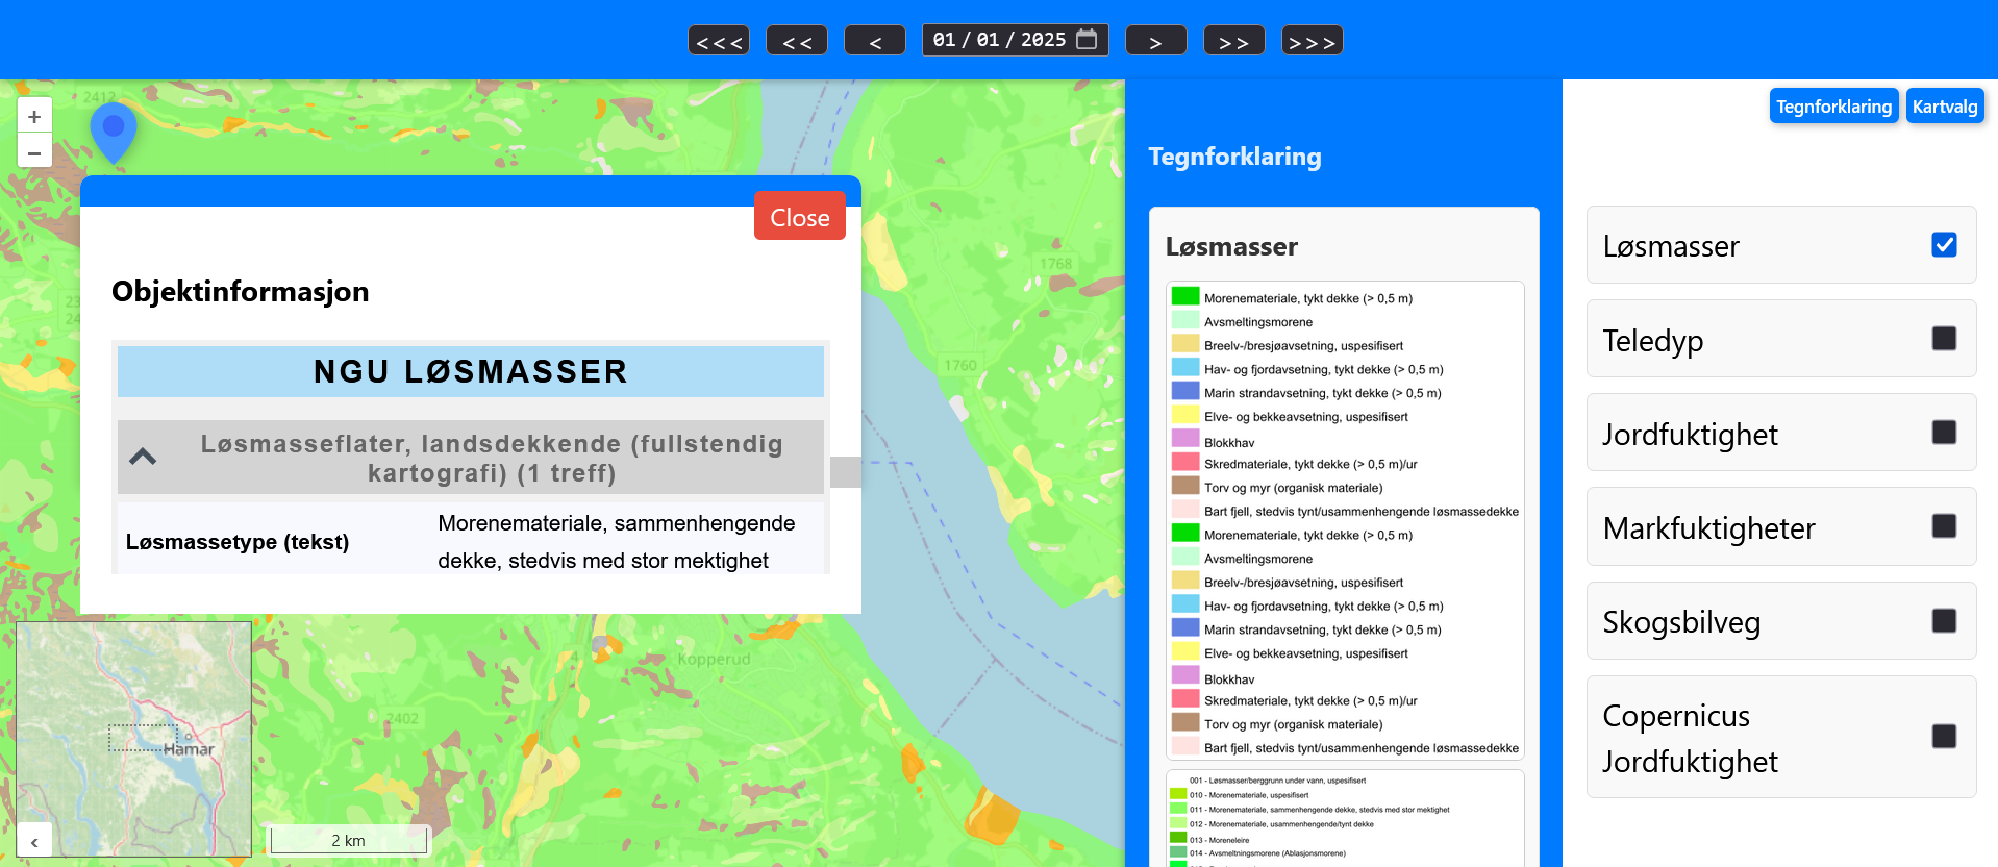
\includegraphics[width=1\linewidth]{figures/website_layout_v1.pdf}
    \caption{Early version of website}
    \label{fig:website_layout_v1}
\end{figure}

\subsubsection*{Final User Interface}

The final version of the \acrshort{ui} represents the \acrfull{mvp} and delivers the core functionality of the application.

As shown in \autoref{fig:website_layout_final}, several aesthetic and usability improvements were made. Icons were added to interface elements, such as chevron icons for the date picker at the top of the page, improving clarity and consistency. The base layer buttons in the bottom-left corner were updated with background images to visually indicate what each layer represents, making it easier for users to select the desired base map.

Based on feedback from the \gls{productowner}, a new feature was introduced to allow users to configure thresholds used to calculate the trafficability of forestry roads. This functionality was implemented in a new sidebar, following the same design as the existing sidebars for layer selection and legends. In this configuration sidebar, users can adjust parameters such as soil saturation and frost depth thresholds. As mentioned earlier, only the forestry road layer supports querying. This design choice simplified the user interface by focusing interactions on the most relevant layer. An example of the query result is shown in \autoref{fig:website_layout_final_sidebars}, where detailed information about a selected road segment is displayed.

To further improve usability, tooltips were added to interactive buttons, providing users with contextual hints about each element's purpose when hovered over.

The interface is primarily designed for desktop use, with layout and controls optimized for larger screens. While some functionality may be accessible on mobile devices, full responsiveness and mobile compatibility were not prioritized in this version.

\begin{figure}[h]
    \centering
    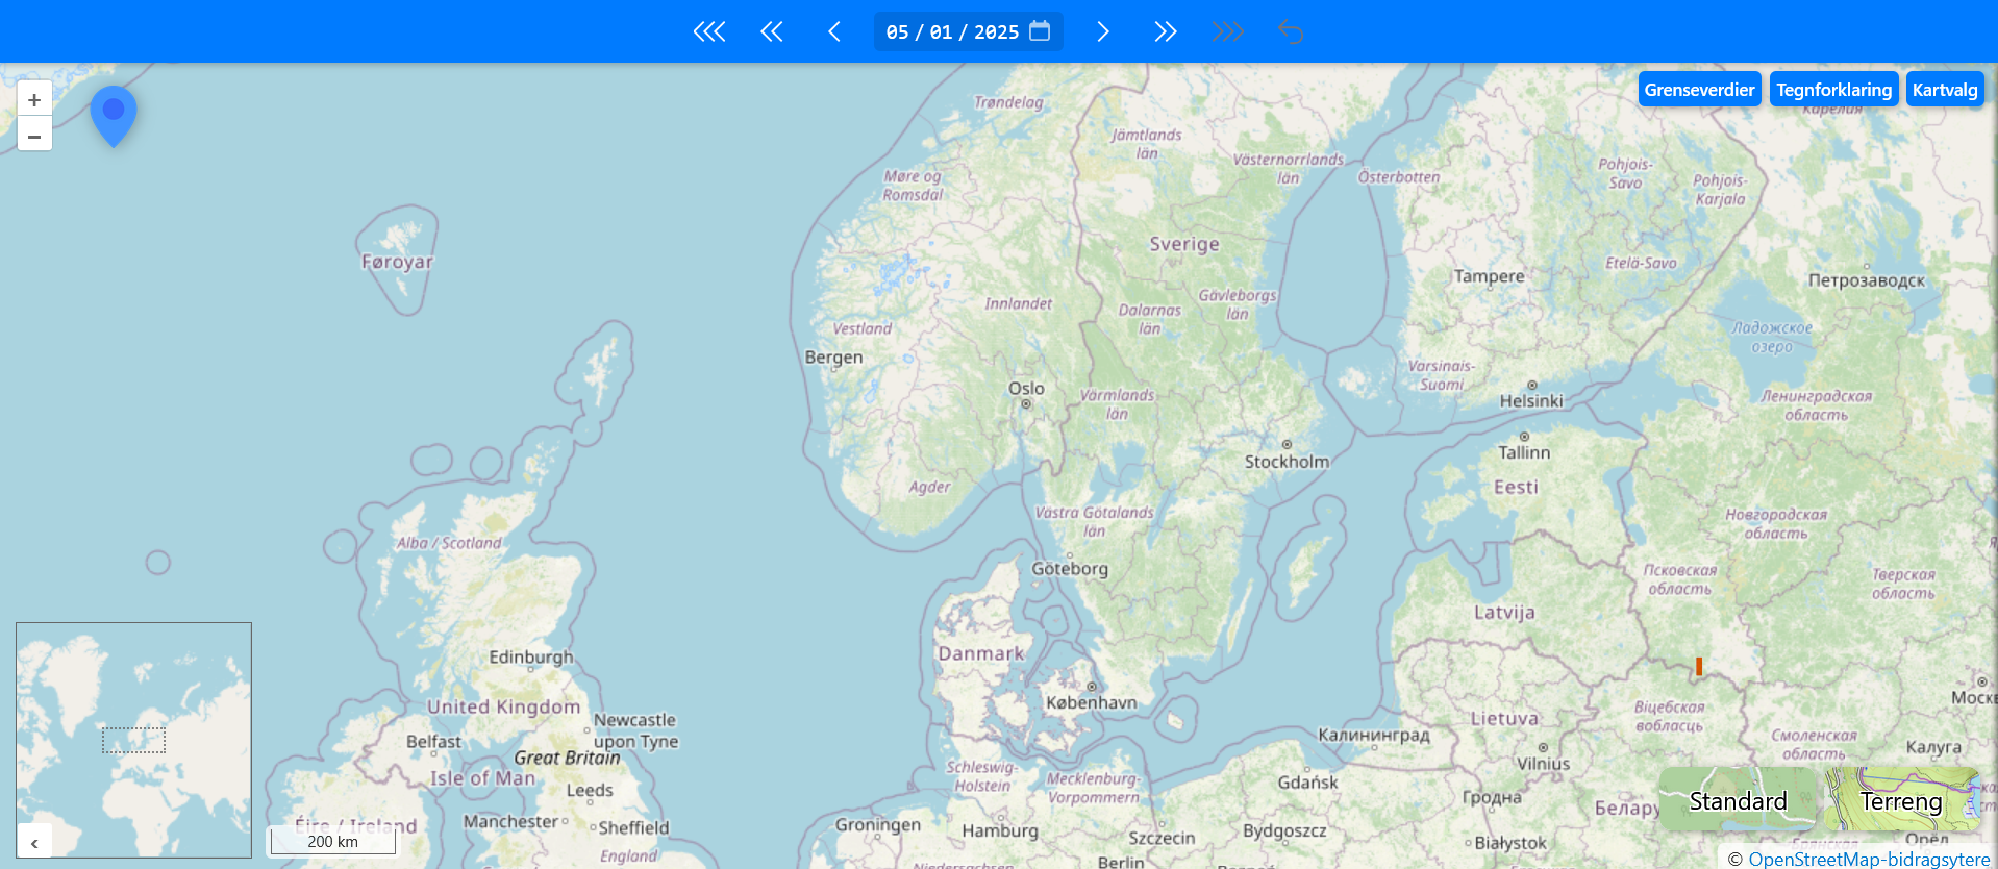
\includegraphics[width=1\linewidth]{figures/website_layout_final.pdf}
    \caption{Final version of website}
    \label{fig:website_layout_final}
\end{figure}

\begin{figure}[h]
    \centering
    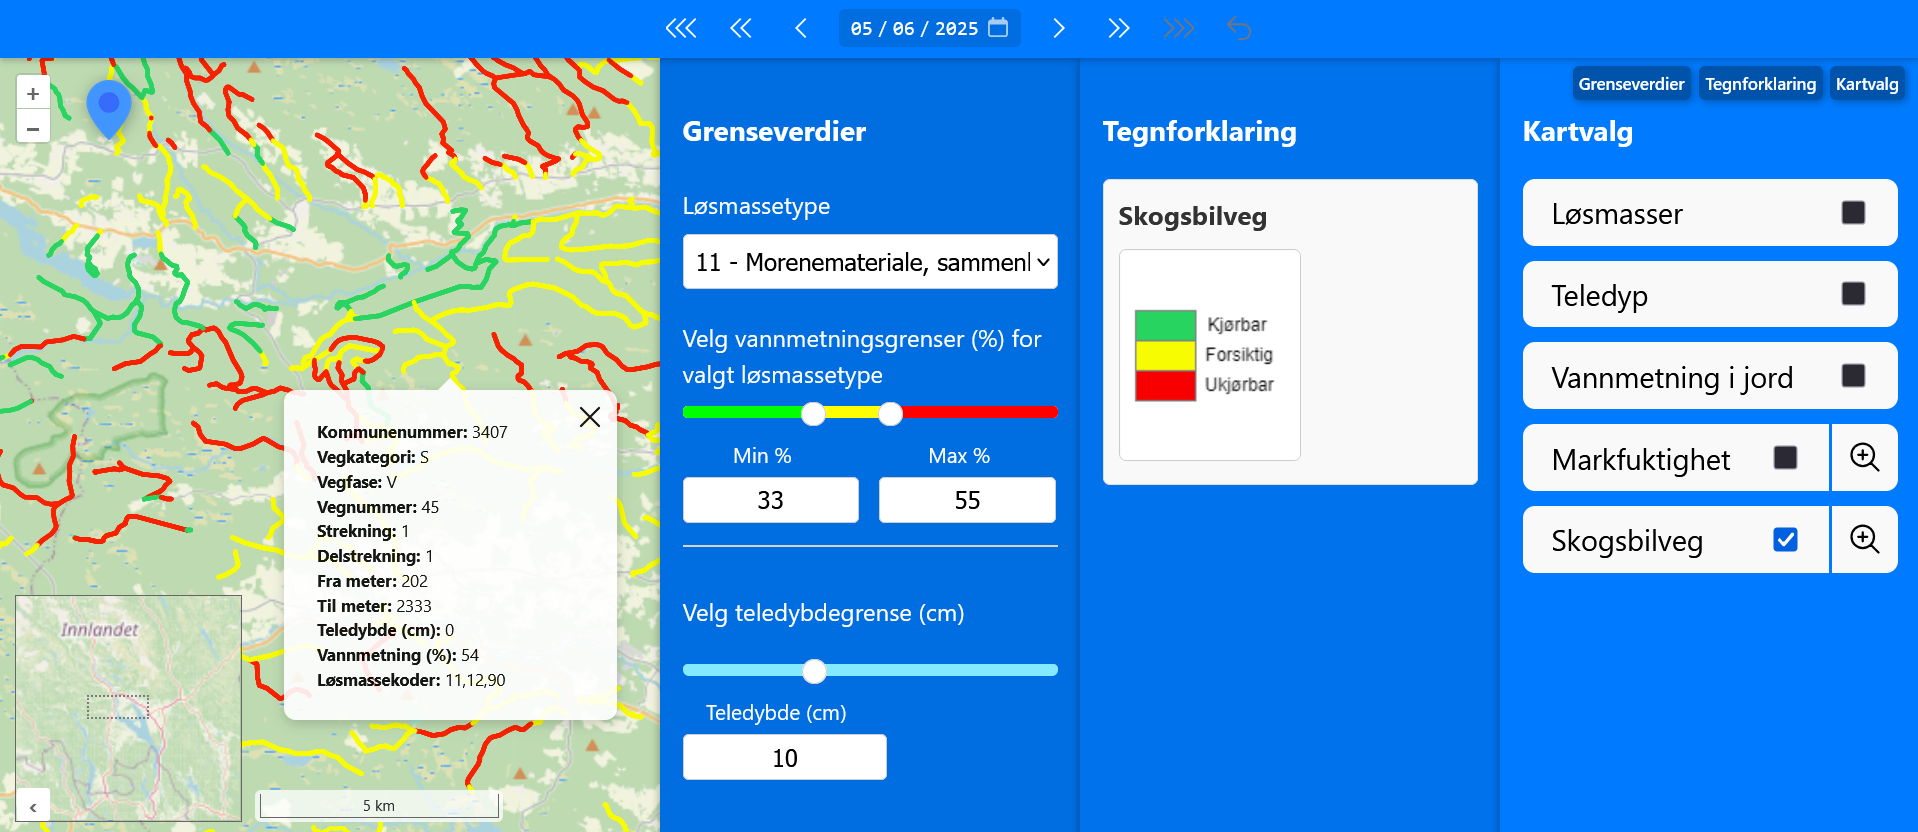
\includegraphics[width=1\linewidth]{figures/website_layout_final_sidebars.png}
    \caption{Final version of website with the sidebars opened}
    \label{fig:website_layout_final_sidebars}
\end{figure}


\subsection{Components}

As described earlier in \autoref{subsec:implementation:technologies:react}, the \acrshort{ui} is composed of multiple React components. While React allows for the reuse of pre-built components, in this application, all components were custom-built to suit specific requirements, except for a few controls provided by OpenLayers. React supports both class and function components, but for this project, we exclusively used function components. These are functions that receive props as input parameters from a parent component, and return TSX markup. Props are useful when a component requires data or functionality from its parent. TSX is a syntax extension similar to \acrshort{html}, but designed to be embedded within TypeScript functions \cite{react_component}.

\autoref{lst:react_component_example} shows an example of a React function component where the OpenLayers map instance is passed as a prop. This design makes it easy to integrate the component into the map, enabling communication between the component and the map. The component returns TSX markup, where the syntax distinguishes between standard HTML elements (e.g., \texttt{<div>}) and custom React components (e.g., \texttt{<ToggleLayers .../>}), the latter identified by their capitalized names. As shown in the example, components can also be nested within other components, allowing for a modular and hierarchical structure.

\begin{figure}[h]
\lstinputlisting[
    caption={Example of a React component},
    label={lst:react_component_example}
]{listings/component_example.tsx}
\end{figure}

When a user interacts with a component, it often needs to update in response. In React, this is handled using what is known as a component's state. Unlike regular variables, state values are preserved across re-renders. State can also be shared between components, a common and effective approach is to store the state in a parent component and pass it down to child components via props \cite{react_state}.

In \autoref{lst:react_state_example}, the \texttt{mapInstance} state is declared using the \texttt{useState} hook. This hook returns a pair: the current state value (\texttt{mapInstance}) and a function to update it (\texttt{setMapInstance}). In this example, an OpenLayers map instance is created and stored in the \texttt{mapInstance} state. This state can then be accessed and modified by other components that interact with the map by setting the state as their props.

\begin{figure}[h]
\lstinputlisting[
    caption={Example of a React state},
    label={lst:react_state_example}
]{listings/state_example.tsx}
\end{figure}

While state enables components to store and update values across renders, many interactive behaviors require performing actions as side effects. In React, such logic is handled using the \texttt{useEffect} hooks. This hook is a function that enables developers to run specific code after the component has rendered, and to react to changes in props, state, or other variables \cite{react_useEffect}.

A common use case for \texttt{useEffect} is to synchronize a component's state with external systems or APIs, in this case, synchronizing React state with the visibility of OpenLayers map layers. The effect shown in \autoref{lst:react_effect_example} monitors changes to the visibility state array and ensures that the corresponding OpenLayers layers are updated accordingly.

\begin{figure}[h]
\lstinputlisting[
    caption={Example of React \texttt{useEffect}},
    label={lst:react_effect_example}
]{listings/effect_example.tsx}
\end{figure}

\subsection{Date Picker}

An important feature requested by the \gls{productowner} was the ability to view forecasts of road trafficability. To support this, a date picker component was implemented, allowing the user to change the date for the data shown on the map.

The date picker consists of a standard \acrshort{html} date input element, along with buttons that increment or decrement the selected date by a day, a week, or a year. When the user selects a new date, all active map layers are re-queried and updated to reflect the data available for the new date. Only layers with available data for the selected date will be shown.

The dynamic data sources include historical data dating back to September 1, 1957, and forecast data extending nine days into the future. To prevent invalid selections, the date picker is restricted to this available date range.

\subsection{Map Integration with OpenLayers}

The interactive map component of the website was implemented using the OpenLayers library. The map was initialized within a custom React component, with its lifecycle managed using React hooks to ensure proper mounting and cleanup. The following types of layers were used:

\begin{itemize}
    \item \textbf{TileLayer}: Used for base map layers. It loads map images in small tiles, improving performance by enabling parallel loading and caching.
    \item \textbf{ImageLayer}: Used for dynamically changing map layers, such as those reflecting date-specific data. Unlike \texttt{TileLayer}, \texttt{ImageLayer} avoids inconsistencies caused by tiles loading at different times.
    \item \textbf{VectorLayer}: Used for client-side rendering of forestry roads from \gls{geojson} data. This layer type enables enhanced interactivity, styling, and feature manipulation.
\end{itemize}

\autoref{lst:wms_example} shows how an \texttt{ImageLayer} is implemented using a WMS source. To specify the WMS source we create a new \texttt{ImageWMS} object which holds values for the URL and the parameters (\texttt{params}). Together these make the full URL used to retrieve the images from the external WMS servers via the backend server.

The map layers are exported from their definition modules. This allows other React components to dynamically control aspects such as layer visibility or update parameters like changing the date of the map layer.

\begin{figure}[h]
\lstinputlisting[
    caption={Example of WMS implementation},
    label={lst:wms_example}
]{listings/openlayers_wms.tsx}
\end{figure}

\subsection{Trafficability Algorithm}\label{subsec:implementation:website:trafficability_algorithm}

As described earlier in \autoref{sec:technicaldesign:website}, the main feature of the website is to visualize forestry roads using a color-coded system: green, yellow, or red, to indicate their current trafficability.
These classifications are based on an algorithm that incorporates both meteorological and geological data.

Initially, we planned to perform these calculations on the backend to maintain cohesion and centralized control over the classification logic. By keeping all data processing on the server, we could ensure that the logic was consistent, easier to maintain, and independent of client-side variations. However, later in the project, the \gls{productowner} requested that users should be able to adjust threshold values for certain parameters dynamically using sliders. Since this would require recalculating the classifications in real time as the slider values changed, it became more efficient to move the algorithm to the frontend. This avoided repeated requests to the backend for each slider adjustment, as the map layer would only need to be fetched once and then re-styled dynamically on the client side.

As shown in \autoref{lst:forestryroads_styling}, each feature rendered on the map includes \gls{geojson} properties for relevant meteorological and geological data, specifically, frost depth, soil saturation, and superficial deposit type. These values are compared against the threshold values selected by the user to determine the color used for each road segment.

The function that determines the color of the road is shown in \autoref{lst:trafficability_algorithm}. If the frost depth exceeds the threshold, the road is classified as having good trafficability (green). If not, the soil saturation value is used to determine whether the trafficability is moderate (yellow) or poor (red), based on user-defined minimum and maximum thresholds.

\begin{figure}[h]
\lstinputlisting[
    caption={Styling of forestry roads},
    label={lst:forestryroads_styling}
]{listings/forestryroads_styling.ts}
\end{figure}

\begin{figure}[h]
\lstinputlisting[
    caption={The trafficability algorithm},
    label={lst:trafficability_algorithm}
]{listings/trafficability_algorithm.ts}
\end{figure}

\subsection{Integration with Backend}

All map data displayed on the website is fetched through the backend server. Each map layer is implemented using an OpenLayers object that sends requests to a specified URL. The response format depends on the type of map layer.

As shown in \autoref{lst:url_example}, \texttt{TileLayer} and \texttt{ImageLayer} use either an XYZ tile URL or a \gls{wms} URL, both of which return rendered map images. In contrast, \texttt{VectorLayer} uses a \gls{wfs} URL to request raw vector features, which is returned in the \gls{geojson} format.

\begin{figure}[h]
\lstinputlisting[
    caption={Example of OpenLayers URL configurations},
    label={lst:url_example}
]{listings/openlayers_url_examples.tex}
\end{figure}

To improve performance and reduce unnecessary network traffic, layers are loaded dynamically based on the user's interaction with the map, such as panning or zooming. Certain layers are only activated at specific zoom levels or within a defined spatial extent to ensure efficient resource usage.

\section{Server}\label{sec:implementation:server}

This section describes the implementation of the server, which serves as the source of information for the website. Additionally, key functionality and iterations will be outlined. The backend server consists of two main parts: a proxy for \Gls{wms} services and an endpoint for the forestry road algorithm. 

\subsection{Forestry Road Algorithm}\label{subsec:server:forestroadalgorithm}

\textcolor{orange}{
Hva det er (api, (REST?)) \\
Hvordan den funker (Hente veidata, cluster, query, send tilbake) \\
Hvorfor vi gjorde det slikt (kanskje ikke? \\
Skrive at vi gikk ut ifra at veiene er lagd av løsmassene i området. Kanskje skrive om de andre... 
) \\
FJORDKATALOG
}

... An overview of the external libraries used is shown in \autoref{tab:golibraries}. ...

\begin{table}[h]
    \centering
    \begin{tabular}{|l|l|}
        \hline
        \textbf{Library} & \textbf{Description} \\
        \hline
        joho/godotenv & Loads environment variables from .env files. \\
        rs/zerolog & Zero Allocation Logger. \\
        tidwall/rtree & R-tree implementation for spatial querying. \\
        twpayne/go-geom & Efficient geometry types for geospatial applications. \\
        twpayne/go-shapefile & Native Go reader for ESRI Shapefiles \\
        \hline
    \end{tabular}
    \caption{Overview of used Go libraries}
    \label{tab:golibraries}
\end{table}

\subsection{Proxy}\label{subsec:server:proxy}

As described in \autoref{sec:systemarchitecture}, we wanted a clean architecture where all requests are routed through the backend server. The implementation of this idea is the proxy endpoint on the server. Proxies are loaded from a JSON\footnote{\url{https://www.json.org/}} file, where each key denotes a specific proxy endpoint, and the corresponding value specifies the target URL to which requests should be forwarded. \autoref{lst:proxycreation} shows how the proxy endpoints are loaded, in addition to the creation of two endpoints for routing the base map layer requests. 

\begin{figure}[h]
\lstinputlisting[
    caption={Creation of proxy endpoint},
    label=lst:proxycreation
]{listings/proxycreation.go}
\end{figure}

\subsection{Optimization}\label{subsec:server:optimization}

Early iterations of the forest road retrieval and processing algorithm were computationally expensive, resulting in long response times when querying the forest road layer.

\subsubsection{SeNorge}\label{subsubsec:implementation:optimization:senorge}

The backend would initially query the SeNorge API once for every road, which would quickly overload the API server leading to long processing times. Additionally, the SeNorge API would not accept multiple coordinates within each grid-cell. SeNorge uses a grid system to divide Norway into \qty{1}{\kilo\meter\squared} cells, and calculate all their climate projections as an average within each cell \cite{senorge_watermap}. 

Lacking documentation of how the grid-cells were initially declared, in addition to a deprecated service for transforming coordinates to cell indexes, prompted further investigation into the SeNorge grid-cells. Findings showed that each grid-cell had borders that lined up with the UTM zone 33N projection system, where the latitude and longitude of each grid intersection were a multiple of \qty{1000}{}. In other words, each grid is centered on a UTM coordinate that is a multiple of $\qty{1000}{}\pm\qty{500}{}$.

The findings made it possible to cluster the forest roads into their closest SeNorge grid-cell, without explicitly knowing which grid-cell was closest. The coordinate of the cluster center could then be used to send a singular request to the SeNorge API, drastically increasing the amount of roads that could be processed at once. Listing \ref{lst:clusterforestroads} shows the implementation of the clustering, where the forest roads are clustered into a sharded map for fast concurrent read and writes.

\begin{figure}[h]
\lstinputlisting[
    caption={Clustering of forest roads},
    label=lst:clusterforestroads
]{listings/clusterwfsresponsetoshardedmap.go}
\end{figure}

\subsubsection{Spatial querying}

Another large optimization was made related to how superficial deposit along the roads were queried. Initially, the middle of each road would be used to query NGU's \Gls{wms} server\footnote{\url{https://geo.ngu.no/kart/losmasse_mobil/}}, leading to a large amount of HTTP requests. These HTTP requests would then quickly overload the \Gls{wms} server, leading to extensive response times.

This was solved by downloading the superficial deposit data and reconstructing it into a map in-memory. The data was downloaded from GeoNorge\footnote{\url{https://kartkatalog.geonorge.no/}} and is available under the NLOD license\footnote{\url{https://data.norge.no/nlod/no/2.0}}. The reconstruction of the spatial data can be found in \autoref{lst:spatialindex}, where each record is read and reconstructed into an R-tree. An R-tree allows for effective querying of spatial data by grouping nearby objects and represent them with their bounding box in the next higher level of the tree \cite{rtreewikipedia}. Having the spatial data in-memory allowed for a greater number of queries along the road.

\begin{figure}[h]
\lstinputlisting[
    caption={Building of spatial index},
    label=lst:spatialindex
]{listings/readshapefileandbuildindex.go}
\end{figure}

\subsubsection{Goroutines}

As previously stated in \autoref{subsec:implementation:technologies:go}, Go was chosen partly due to its native concurrency functionality. This proved to be a wise decision, as Goroutines was a large part of reducing the processing times. The amount of features (forestry roads) shown on the map at once can range from zero to several thousands, depending on the zoom level used. Processing these sequentially would lead to extensive processing times, whereas use of parallel processing ensured consistently low loading times, even when handling large volumes of data. An example of how Goroutines was used can be seen in \autoref{lst:clusterforestroads}, where a wait-group and a semaphore are used to synchronize and limit the amount of Goroutines used.

\begin{comment}
UTFORDRINGER OM IMPLEMENTASJON HER:
    - Kilder
        - Senorge dårlig dokumentasjon til API
            - Bruker annen endpoint istedenfor
    - Finne gode og nøyaktige data
    - Gjøre om data til WMS/noe vi kan vise
    - Gjøre om WMS/kartdata til rød, grønn eller gule veier
    - Konvertering av koordinater, f.eks. fra epsg:3857 til epsg:25833
    - Klassifisering av skogsbilveger
        - Hente teledyp data for flere veger (WMS vs. REST API)
        - Teletyp var vanskeligere enn forventet siden API-en brukte et dårlig dokumentert grid-system.
\end{comment}
